\section{Virtual Memory}

\begin{frame}[fragile]{Virtual Memory}
	\emoji{bullseye} Why do we need virtual memory?
	\begin{itemize}
		\item Virtual memory is another abstraction layer between process and physical memory.
		      \begin{itemize}
			      \item<1-> \textbf{Isolation}: Each process has its own address space.
			      \item<2-> \textbf{Protection}: Deny the process from accessing other processes' or privileged memory.
			      \item<3-> \textbf{Efficiency}: Support Copy-on-Write, can run a partially loaded program.
		      \end{itemize}
	\end{itemize}

	\onslide<4->{
		\emoji{thinking} How to implement virtual memory?
		\begin{itemize}
			\item We'll only talk about \textbf{Paging} today.
		\end{itemize}
	}

\end{frame}

\begin{frame}[fragile]{Paging in a Nutshell}

	\begin{itemize}
		\item<1-> \textbf{Page and Frame}
		      \begin{itemize}
			      \item Physical memory is split into \textbf{fixed-size frames}.
			      \item Virtual memory is split into \textbf{fixed-size pages}.
		      \end{itemize}
		\item<2-> \textbf{Memory Mapping}
		      \begin{itemize}
			      \item Hardware support: \textbf{MMU} (Memory Management Unit)
			      \item Function: Translate \textbf{virtual page} to \textbf{physical frame}
			      \item Data structure: \textbf{Page Table}
		      \end{itemize}
		\item<3-> \textbf{Page Fault}
		      \begin{itemize}
			      \item If a page is not in physical memory, a page fault occurs.
			      \item The OS will load the page from disk to physical memory, and update the page table.
		      \end{itemize}
	\end{itemize}

\end{frame}

\begin{frame}[fragile]{Paging in practice}

	\begin{columns}
		\begin{column}{0.3\textwidth}
			\begin{figure}[H]
				\centering
				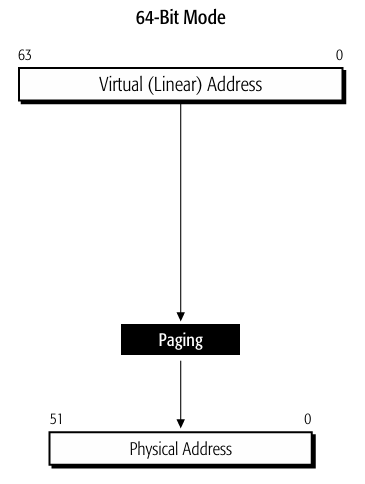
\includegraphics[width=\textwidth]{day3/img/page.png}
			\end{figure}
		\end{column}
		% \onslide<2->{
		\begin{column}{0.7\textwidth}
			\begin{figure}[H]
				\centering
				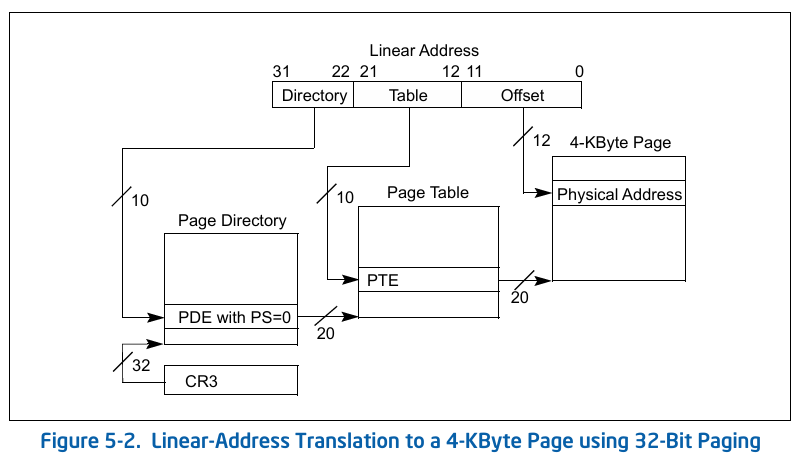
\includegraphics[width=\textwidth]{day3/img/page-table.png}
			\end{figure}
		\end{column}
		% }
	\end{columns}

\end{frame}
